\section{Particle Size Determination}
\label{sec:5.4:ParticleSizeDetermineation}

With assumed particle size distributions for the retrievals aerosol extinction form the previous section there is a unfavour wavelength dependance on the values of the extinction. In this section a discussion of the requirement to achieve full particle size information will be underwent followed by the method used to determine some particle size used on the ALI measurement s and the results with with updated extinction profiles.

\subsection{Particle Size Sensitivity}

To rectify the problem with the dependance between the extinction and wavelength a method will be preformed on the data in order to try to extract some particle size information But first a look into the information of particle size from limb measurements must be explored. From work done by \citep{Rieger2014} shows that different particle size distributions can effect the aerosol measurement vector. He uses an OSIRIS scan geometry and calculates the respective measurement vectors for a series of particle sizes which can be seen in reproduction of \autoref{fig:5.4:AerosolMeasurementParticleSizeInfo}. In panel A three different log-normal distributions are used which give a near identical measurement vector at 750~nm with simulation of the atmosphere with SASKTRAN. The three profiles are in blue is a single fine mode particle size distribution with a mode radius and width of 0.08~\si{\micro\meter} and 1.6 respectively, black is a bimodal particle size distribution the simulates volcanic conditions with the mode radius and width of 0.08~\si{\micro\meter} and 1.6 for the fine mode and 0.4~\si{\micro\meter} and 1.2 for the coarse mode, lastly red is a representative size distribution with mode radius and width of 77~\si{\micro\meter} and 1.75. Panel B shows the measurement vectors calculated with the three distributions across a series of wavelengths. The third panel, panel C, shows the difference of the measurement vectors compared to the bimodal distribution. Sensitivity to particle size is only seen past 800~nm measurement but great sensitivity does not occur until measurement recorded out to 1500~nm. Furthermore an error of 1\% in the radiance yields a relative error in the bimodal distribution measurement vector shown by the gray shading.

\begin{figure}
\centering
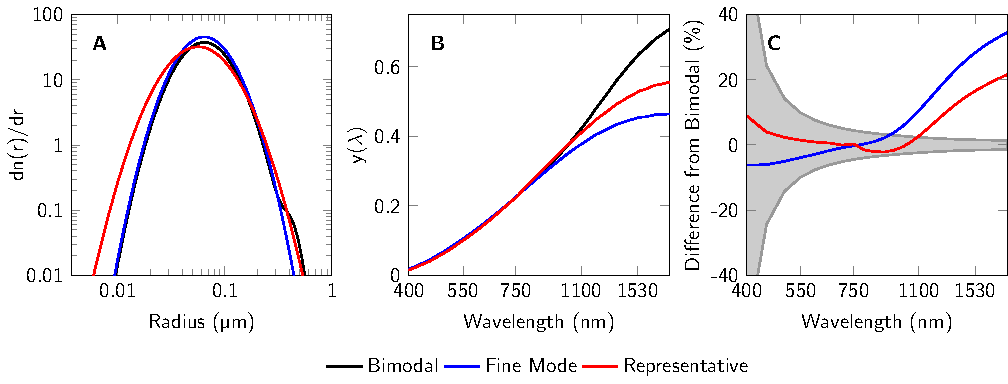
\includegraphics[width=1.0\textwidth]{./Images/5-4-AerosolMeasurementParticleSizeInfo.pdf}
    \caption[Aerosol Measurement Vectors Sensitivity to Particle Size]{Reproduced from \citep{Rieger2014}. For OSIRIS scan 6432001 aerosol measurement vectors were calculated at 22.5~km. (A) The three size distributions used in the study. (B) The measurement vectors calculated via the SASKTRAN simulation (C) The relative percent difference of the fine and representative distributions with respect to the bimodal distribution. A 1\% error is the radiance yields an uncertainty in the bimodal measurement vector shown by the grey shading.}
    \label{fig:5.4:AerosolMeasurementParticleSizeInfo}
\end{figure}

For ALI measurement were only gathered between 650 and 950~nm in wavelength, due to the CCD camera not having the required efficiency sample at wavelengths above this point. As such ALI only has some sensitivity to particle size form the longer wavelengths and only a small amount. As such it is not possible to determine both the mode radius and mode width due to information poor wavelengths. Instead the data from ALI will be used to determine the Angstr\"{o}m exponent. The Angstr\"{o}m exponent is an approximation to Mie scattering since the value of the Angstr\"{o}m exponent, $\alpha$, is an analogy to particle size. The scattering cross section for aerosol is dependant the particle size distribution assuming since the number density must be a constant across wavelength, as such the extinction value changes with a change in cross section. From \autoref{eqn:5.4:agstromCoefficient} the particle size profile from a series wavelength can be determined from the Angst\:{o}m exponent.Lower Angstr\"{o}m exponents correspond to larger particle sizes and vice versa for small particle sizes. Since the measurements observe relatively the same atmosphere over the time of one complete aerosol cycle; the differences between extinction ratios at the different wavelength can be used to gather a understanding of aerosol particle size in the form
\begin{equation}
    \frac{n\sigma}{n_{0}\sigma_{0}} = \left(\frac{\lambda}{\lambda_{0}}\right)^{-\alpha}
    \label{eqn:5.4:agstromCoefficient}
\end{equation}
where $n$ is the aerosol concentration, and $\sigma$ is the scattering cross section. For the 750~nm wavelength for a variety of mode radius and widths a change in the cross section can be observed in \autoref{fig:5.4:scatteringCrossSections}. The Angstr\"{o} exponent can also be determine  fitting a line through a series of points by rearangeing \autoref{eqn:5.4:agstromCoefficient} into the following
\begin{equation}
    \alpha = -\frac{\log(n\sigma)-\log(n_{o}\sigma_{o})}{\log(\lambda)-\log(\lambda_{o})}
    \label{eqn:5.4:agstromCoefficientSlope}
\end{equation}
which show the Anstr\"{o}m exponent in simple the slope of the log of the extinction over the log of the wavelengths.

\begin{figure}
\centering
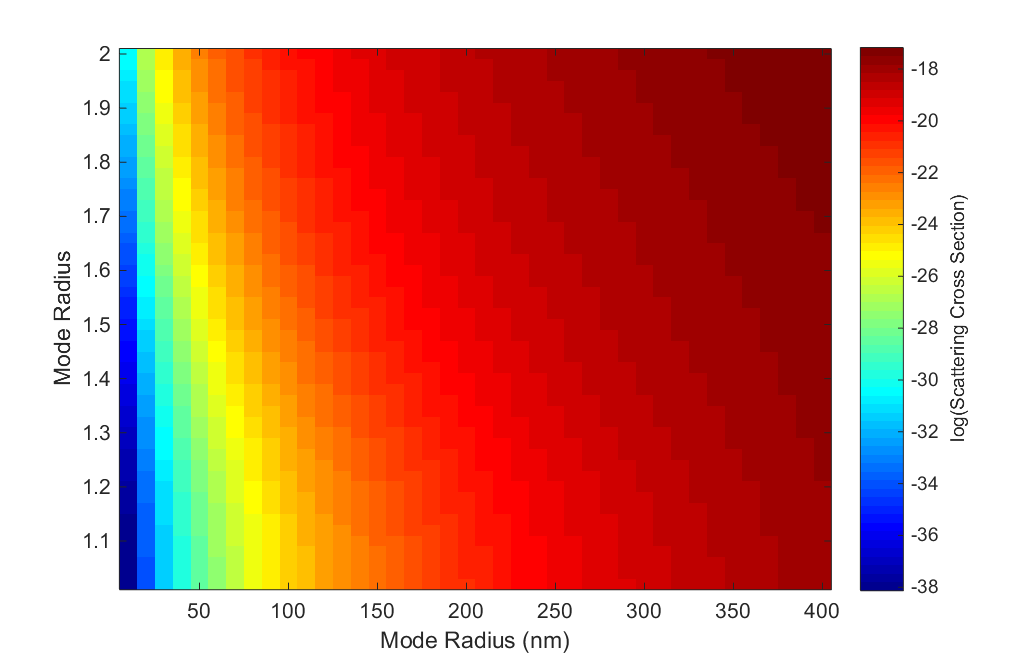
\includegraphics[width=1.0\textwidth]{./Images/5-4-CrossSectionDependance.pdf}
    \caption[Log of Scatting Cross Section for Various Mode Radii and Widths]{Computed with the optical properties of the SASKTRAN engine. This varation of the corss section with respect to the mode radius and width allows for some determination of the particle size distribution through the Angstr\:{o} exponent.}
    \label{fig:5.4:scatteringCrossSections}
\end{figure}

\subsection{Particle Size Retrieval Method and Results}

Once the retrieval has been preformed for a complete series of wavelengths; determination of the Angstr\"{o}m exponent occurs which is preformed in a similar manor as outlined by \cite{Rault2013} for the OMPS aerosol particle size retrieval.  For the retrieval described here a single mode log-normal distribution is assumed with a mode radius, $r_{g}$, and the mode width, $\sigma_{g}$, which is the same as the OSIRIS version 5.07 aerosol product of 0.08\si{\micro\meter} and 1.6 respectively. The process for the retrieval is as follows:
\begin{enumerate}
    \item Set up a MART retrievals for all wavelengths measured by ALI was a mode radius and width of 0.08\si{\micro\meter} and 1.6 respectively.
    \item Preform the MART retrieval for each wavelength.
    \item For all wavelengths determine the maximum minimum retrial altitude and minimum maximum retrieval altitude. These will be the bound for for the particle size retrievals.
    \item For each valid tangent height fit a least squares line through the extinctions and wavelengths via \autoref{eqn:5.4:agstromCoefficientSlope} to determine the Angstr\"{o}m exponent. A wavelength at a altitude was rejected if the forward model at that shell altitude was not within 3\% of the measurement vector.
    \item For each tangent height convert the Angstr\"{o}m exponent into a mode radius assuming a mode width of 1.6.
    \item Take the median of all the determined mode radii and use this as the new values for the mode radius. If this value is the same as the previous iteration stop the retrieval as the solution has converged, If it is different change the mode radius in the model to the new mode radius and repeat the sequence from step 2.
\end{enumerate}
This method generally achieved convergence within 4-5 iterations.

A sample particle size retrieval is shown in \autoref{fig:5.4:ParticleSize} for the cycle consisting of images 204-216. The first panel of \autoref{fig:ParticleSize} shows the median Angstr\"{o}m exponent that was determined after each iteration and convergence can be seen after a couple iterations. The initial guess for the mode radius was changed to several different values and each run of the model resulted in the same final retrieved mode radius. The particle size determined for ALI in the last complete set of aerosol images can be seen in the second panel of \autoref{fig:ParticleSize} which yields a final Angstr\"{o}m exponent of between 2 and 3 throughout the altitude range from 13 to 22~km. Assuming a mode width of 1.6 yields a median mode radius of 0.105~\si{\micro\metre}. The final panel shows the least squares for the 20.5~km tangent altitude for this case only 11 of the 13 possible wavelengths contributed to the determination of the Angstr\"{o}m exponent.

\begin{figure}
\centering
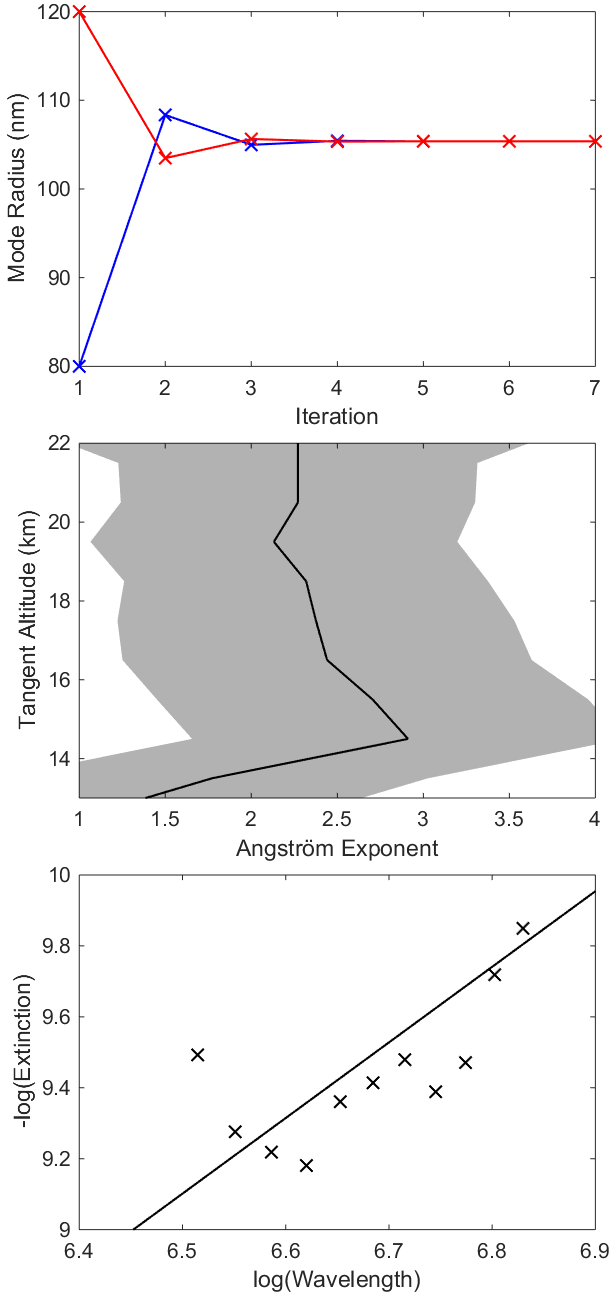
\includegraphics[width=0.5\textwidth]{./Images/5-4-ParticalSize.pdf}
    \caption[Particle Size Retrieval]{The top panel shows the convergence of two sample particle size retrievals over the iterations, blue and red represent a priori of 0.08 and 0.12~\si{\micro\metre} respectively. Both initial state converge to the same value over approximately 4 iteration in the particle size retrieval method. The second panel is the final Angstr\"{o}m exponents determined for images 204-217 during the Timmins 2014 campaign and are in black as the final profile was almost identical after each particle size retrieval, the shading represents the error associated with the least squares fit. The last panel demonstrate a least squares fit to determine the Angstr\"{o}m exponent at 20.5~km shell altitude.}
    \label{fig:5.4:ParticleSize}
\end{figure}

The error in the Angstr\"{o} exponent was determined looking at the error in the slope possible from the least squares method. Assuming no error in the extinction points the error in the slope is given by
\begin{equation}
    \delta\alpha = \frac{s}{SS_{xx}}
\end{equation}
where $s$ is
\begin{equation}
    s = \sqrt{\frac{SS_{yy}-\alpha SS_{xy}}{n-2}},
\end{equation}
and $SS_{xx}$, $SS_{yy}$, and $SS_{xy}$  are the sum of squares of the wavelength, aerosol extinction, and cross term between the wavelength and aerosol extinction and $n$ is the number of points. However there is and associated error with each aerosol extinction profile. To determine the error on the Angstr\"{o}m exponent accounting for the precision in the aerosol extinction the error on the slope was calculated 10,000,000 times with each iteration a random amount of error from he known range was added to each extinction point. Then the mean from the all the errors of the least squares fit was used as the fine precision estimate on the Angstr\"{o}m coefficient which can be seen in the second panel of \autoref{fig:5.4:ParticleSize}.

The extinction cycle similar to \autoref{fig:5.3:AliAerosolCycleNoPartSize} is shown in \autoref{fig:5.4:AliAerosolCycle} except with updated particle size parameters form the retrieval. the aerosol extinction profiles now shows the characteristic decrease in aerosol extinction that is expected as wavelength increase. this extinction is self consistent with Mie theory and give some validity to the retrieved particle sizes determined from ALI.

\begin{figure}
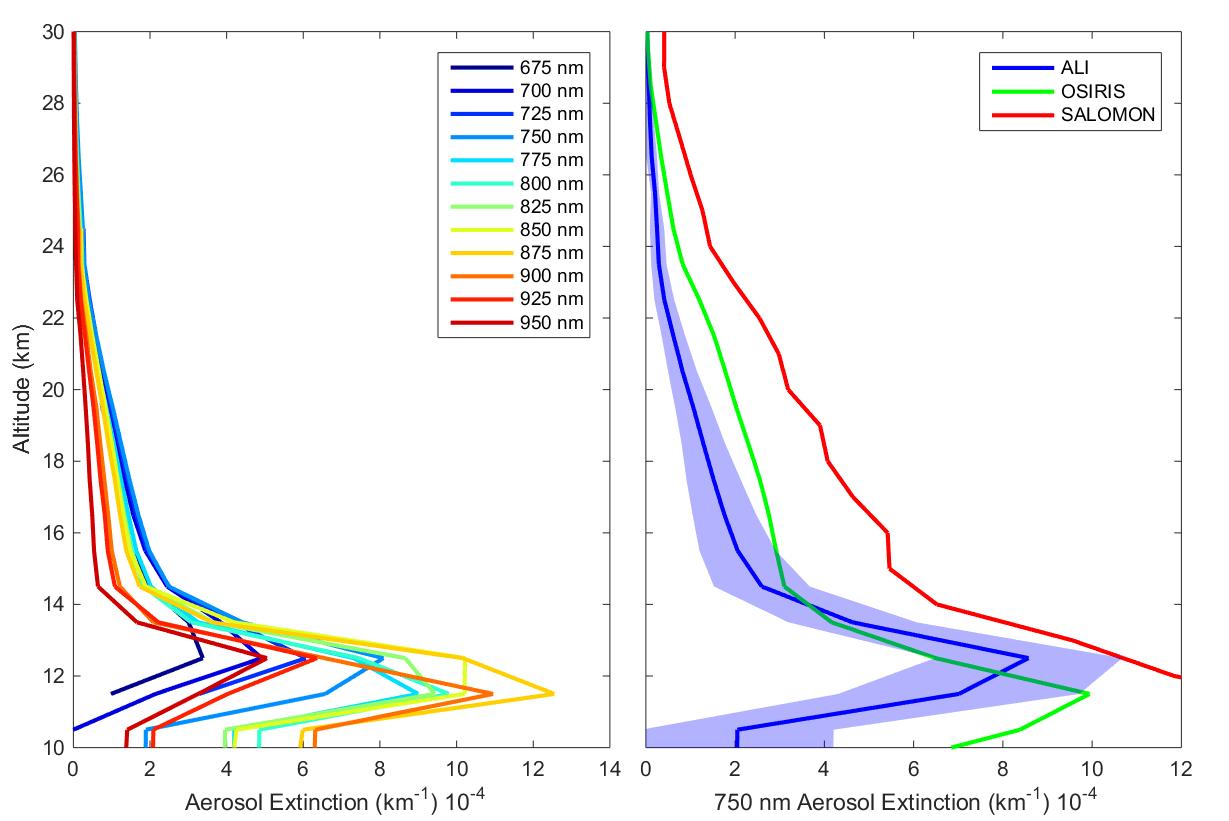
\includegraphics[width=1.0\textwidth]{./Images/5-4-FullAerosolCycleComparison.pdf}
    \caption[Aerosol Retrievals with Corrected Particle Size for All Wavelengths and 750~nm Comparison with OSIRIS and SALOMON]{Left is the retrieved aerosol extinction profiles from the last complete cycle consisting of images 205 to 216 from the 0.0\si{\degree} horizontal line of sight. Right is the 750~nm ALI aerosol extinction in blue with its error represented by the shading compared to the 750~nm extinction measured by OSIRIS and SALOMON in green and red respectively.}
    \label{fig:5.4:AliAerosolCycle}
\end{figure}   